\chapter{System Modelling}
\label{system_modelling}

\emph{This chapter gives a mathematical description of the component modelling. Thus the different physical and mathematical measures of hydraulic systems are introduced. The similarities to electronic network modelling are shown by explaining the relevant properties of graph theory. A reduced model for multi-inlet networks is first introduced, then the inclusion of tanks is discussed. In the end, the EPANET-based modelling approach is introduced and compared to the real-world system.}

\section{Hydraulic component modelling}
\label{hydraulic_component_modelling}

In this section the mathematical relation between pressure and flow is given for each component in a WSS system, in order to show their non-linear behaviour. The purpose here is not to derive the different models, rather to introduce the mathematical formalism which describes them.

\eqref{onecomponent} shows the dual variables which describe all two-terminal components in the network 

\begin{equation}
\label{onecomponent}
 \begin{bmatrix}
    \Delta p \\
    q
\end{bmatrix}
=
 \begin{bmatrix}
    p_{in} - p_{out} \\
    q
\end{bmatrix},
\end{equation}

 \begin{minipage}[t]{0.20\textwidth}
where\\
\hspace*{8mm} $\Delta p$ \\
\hspace*{8mm} $q$ \\
\hspace*{8mm} $p_{in}$, $p_{out}$ 
\end{minipage}
\begin{minipage}[t]{0.68\textwidth}
\vspace*{2mm}
is the differential pressure across the element,\\
is the flow through the element,\\
are the absolute pressures.
\end{minipage}
\begin{minipage}[t]{0.10\textwidth}
\vspace*{2mm}
\textcolor{White}{te}$\unit{m}$\\
\textcolor{White}{te}$\unit{m}$\\
\textcolor{White}{te}$\unit{\frac{l}{s}}$
\end{minipage}

\subsection{Pipe model}
\label{pipe_component}

Pipes in the network are governed by the dynamic equation

\begin{equation}
\label{complete_pipemodel}
  \Delta p_i = J_i \dot{q_i} + f_i(q_i) - \Delta h_i,
\end{equation}

 \begin{minipage}[t]{0.20\textwidth}
where\\
\hspace*{8mm} $J_i$ \\
\hspace*{8mm} $f_i(q_i)$ \\
\hspace*{8mm} $\Delta h_i$ 
\end{minipage}
\begin{minipage}[t]{0.68\textwidth}
\vspace*{2mm}
is the mass inertia of the pipes,\\ 
is the pressure drop due to friction,\\
is the pressure drop due to geodesic level difference across the two terminals of pipe elements.
\end{minipage}

The dynamics of the pipes are discarded in the project, as it is shown in other works that the small time constant of the pipe dynamics are not dominant in the system, especially if there are elevated reservoirs included \cite{8thsemester_project,kenneth_houe}. Therefore the pressure across pipes can be written as


\begin{equation}
\label{complete_pipemodel1}
  \Delta p_i = f_i(q_i) - \Delta h_i,
\end{equation}

The pressure drop due to friction across the $i^{th}$ edge is a diagonal map where $f: \mathbb{R}^{m} \rightarrow \mathbb{R}^{m} $ is strictly increasing.\footnote{A map $f: \mathbb{R}^{m} \rightarrow \mathbb{R}^{m} $ is strictly increasing if $\langle x-y, f(x)-f(y) \rangle > 0$ for every $x,y \in \: \mathbb{R}^{m}$ such that $x \neq y$ \cite{oneinput_paper}.} As it is shown in \eqref{deltap_friction}, $f_i$ describes a flow dependant pressure drop due to the hydraulic resistance

\begin{equation}
  \label{deltap_friction}
  f_i(q_i) = \rho_i |q_i|q_i,
\end{equation}

 \begin{minipage}[t]{0.20\textwidth}
where\\
\hspace*{8mm} $\rho_i > 0$ 
\end{minipage}
\begin{minipage}[t]{0.68\textwidth}
\vspace*{2mm}
is the parameter of the pipes. 
\end{minipage}

The form in \eqref{deltap_friction} is motivated by turbulent flow in the pipes in the network, which is typical in water supply applications\cite{prahata}. In the following sections it is assumed that each $f_i$ has a structure shown in \eqref{deltap_friction}.

It is important to note here that $f_i(\cdot)$ is a homogeneous map which means that if the argument is multiplied by a scalar, then its value is multiplied by some power of this scalar \footnote{$g(\alpha v) = \alpha^k g(v)$}. For $f_i(q_i)$, it can be shown that

\begin{equation}
  \label{homogeneity}
  \rho_i |(\alpha q_i)|(\alpha q_i) = f_i(\alpha q_i) = \alpha^2 f_i(q_i).
\end{equation}

This property is noted here and used later in the system description, in \secref{multi_inlet_reduced_network_description}.

\subsection{Valve model}
\label{valve_component}

Valves in the network are governed by the following algebraic expression

\begin{equation}
\label{valvemodel}
 \Delta p_i = \mu_i(q_i,k_v) = \frac{1}{k_v(OD)^2} |q_i| q_i, 
\end{equation}

 \begin{minipage}[t]{0.20\textwidth}
where\\
\hspace*{8mm} $k_v$ 
\end{minipage}
\begin{minipage}[t]{0.68\textwidth}
\vspace*{2mm}
is the valve conductivity function, taking in its argument the Opening Degree(OD) of the valve \cite{8thsemester_project}.
\end{minipage}

$\mu_i(q_i,k_v)$ is a continuously differentiable and proper function which for $q_i = 0$ is zero and monotonically increasing.

\subsection{Pump model}
\label{pump_component}

Centrifugal pumps are governed by the following expression \cite{kallesoePHD}

\begin{equation}
  \Delta p = -a_{h2}{q_i}^2 + a_{h1} \omega_r q_i + a_{h0}{\omega_r}^2
  \label{eq:PumpModel}
\end{equation}

\begin{minipage}[t]{0.20\textwidth}
where\\
\hspace*{8mm} $\Delta p$ \\
\hspace*{8mm} $a_{h2}$,$a_{h1}$,$a_{h0}$ \\
and \hspace*{0.7mm} $\omega_r$ 

\end{minipage}
\begin{minipage}[t]{0.68\textwidth}
\vspace*{2mm}
is the differential pressure produced by the pump,\\
are constants describing the pump,\\
is the impeller rotational speed.
\end{minipage}
\begin{minipage}[t]{0.10\textwidth}
\vspace*{2mm}
\textcolor{White}{te}$\unit{head}$\\
\textcolor{White}{te}$\unit{\cdot}$\\
\textcolor{White}{te}$\unit{\frac{rad}{s}}$
\end{minipage}  

\subsection{Elevated reservoir model}
\label{elevatedreservoir_component}

In elevated reservoirs, the rate of change in the volume of the fluid inside the tank is equal to the volumetric flow at which water enters or leaves the tank. Since the pressure on the bottom is due to the cross sectional area of the tank and the amount of water in it, proportional relation can be set between the pressure and the flow in and out of the tank. The dynamics of such a system can be described by a first order differential equation of the form

\begin{equation}
\label{wt_model}
\dot{p}_i = -\tau_i\Big(\frac{p_i}{h_i}\Big) q_i
\end{equation}

 \begin{minipage}[t]{0.20\textwidth}
where\\
\hspace*{8mm} $p_i$ \\
\hspace*{8mm} $h_i$ \\
\hspace*{8mm} $\tau_i$ \\
\newline
\hspace*{8mm} $q_i$ 
\end{minipage}
\begin{minipage}[t]{0.68\textwidth}
\vspace*{2mm}
is the pressure at the node connected to the tank,\\ 
is the water level in the tank,\\ 
is a parameter dependant of the cross sectional area of the tank,\\
is the flow in the tank if $q_i > 0$ and flow out of the tank if $q_i < 0$.
\end{minipage}

As can be seen in \eqref{wt_model}, in general, the parameter of the tank depends on the pressure and water level ratio, if the cross sectional are is not constant along the height of the tank. However, it is assumed that tanks have the same cross sectional areas in the entire height. Then \eqref{wt_model} simplifies to

\begin{equation}
\label{wt_model}
\dot{p}_i = -\tau_i q_i.
\end{equation}

\section{Graph-based network modelling}
\label{graph_based_network_modelling}

Graph-based network modelling has the advantage of making use of tools from circuit theory. Most of these tools are developed based on Graph Theory(GT). These methods can be used to model WSSs as directed graphs, where components of the systems, such as valves, pipes, tanks and pumps can correspond to edges and each terminal of the network correspond to nodes, or equivalently, to vertices.

In case of WSSs, in order to track the pressure and flow in the desired part of the network, the equation system of the network has to be solved for the desired edges and vertices. The whole network can be described by writing up the equations for all edges in the network, based on the mathematical modelling of the different components in the system, as shown in \secref{hydraulic_component_modelling}. However, in case of complex systems as water networks for large cities, these systems of equations are difficult to handle individually and typically cannot be solved explicitly if there are loops in the system. Therefore the properties of GT are not only useful for setting up relations between flow and pressure, but to make handling of a algebraic constraints easier by exploiting the properties of the matrix algebra. Thereby making it convenient for implementing it in computer algorithms for iterative solving methods.  

WSSs can be described by a directed and connected graph, such that \cite{graph_intro}: 

\begin{equation}
  \label{Numberofchords}
  \mathcal{G} = \{\mathcal{V}, \mathcal{E} \} ,
\end{equation}

\begin{minipage}[t]{0.2\textwidth}
where\\
\hspace*{8mm} $\mathcal{G} $ \\
\hspace*{8mm} $\mathcal{V} $ \\
\hspace*{8mm} $\mathcal{E} $
\end{minipage}
\begin{minipage}[t]{0.68\textwidth}
\vspace*{2mm}
is a directed and connected graph,\\
is the set of vertices, where $\mathcal{V} = \{v_1, ..., v_n\}$,\\
is the set of edges, where $\mathcal{E} = \{e_1, ..., e_m\}$. 
\end{minipage}

\subsection{Incidence matrix}
\label{incidence_matrix}

The incidence matrix, $H$, of a connected graph, $\mathcal{G}$, is a matrix where the number of rows and columns correspond to the number of vertices and edges, respectively. Therefore $H\in \: \mathbb{R}^{n \times m}$. In case of hydraulic networks, edges are directed in order to keep track of the direction of the flow in the system. 

\begin{equation}
\label{DiGraph}
 H_{i,j} =
		\left\{
		\begin{array}{ll}
		
		1 			&      \text{if the $j^{th}$ edge is incident out of the $i^{th}$ vertex}.	
\\
	    -1          &      \text{if the $j^{th}$ edge is incident into the $i^{th}$ vertex}.
\\
        0           &      \text{if the $j^{th}$ edge is not connected to the $i^{th}$ vertex}.

		\end{array}
		\right.
\end{equation}	

It is worth mentioning that the reduced incidence matrix can be obtained by removing any arbitrary row from $H$. Therefore $H$ always have $(n-1)$ row rank. This statement can be explained by the mass conservation in the network, which is explained in the following section, \secref{kirchhoffs_law}.

\subsection{Cycle matrix}
\label{cycle_matrix}

Purely tree structure of a WSS is not common when considering water distribution systems. However, trees can be arbitrarily chosen from the underlying graph of the system.\footnote{Recall that a tree with $n$ vertices has $n-1$ edges \cite{deo2017graph}.}  A tree, $\mathcal{T} $, of the graph is a connected sub-graph where any two vertices are connected by exactly one path \cite{deo2017graph}. Therefore a certain sub-graph which is a tree of the network can be represented as follows

\begin{equation}
  \label{Numberofchords}
  \mathcal{T} = \{\mathcal{V_{\mathcal{T}}}, \mathcal{E_{\mathcal{T}}} \} 
\end{equation}

A special case of connected tree sub-graphs is the spanning tree of the network. A spanning tree contains all the vertices of $\mathcal{G}$ and has no cycles, since it is a tree. A spanning tree of the network therefore can be represented as

\begin{equation}
  \label{Numberofchords}
  \mathcal{T} = \{\mathcal{V}, \mathcal{E_{\mathcal{T}}} \} 
\end{equation}

In order to obtain a spanning tree, an edge has to be removed from each cycle. The removed edges are $\mathcal{G} - \mathcal{T}$, and called the chords of $\mathcal{T}$ with respect to $\mathcal{G}$. By adding a chord to $\mathcal{T}$, a cycle is created which is called a fundamental cycle. A graph is conformed by as many fundamental cycles as the number of chords \cite{deo2017graph}.

The set of fundamental cycles correspond to the fundamental cycle matrix, $B$, such that the number of rows and columns are defined by the number of chords and edges, respectively. The cycle matrix of the system is given by

\begin{equation}
\label{DiGraphCycle}
 B_{i,j} =
		\left\{
		\begin{array}{ll}
		
		1 			&     \text{if the $j^{th}$ edge belongs to the $i^{th}$ cycle and their directions agree}	
\\
		-1          &     \text{if the $j^{th}$ edge belongs to the $i^{th}$ cycle and their directions are opposite}
\\
        0           &     \text{if the $j^{th}$ edge does not belong to the $i^{th}$ cycle}
		\end{array}
		\right.
\end{equation}	

\subsection{Kirchhoff's and Ohm's law for hydraulic networks}
\label{kirchhoffs_law}

In this project the hydraulic system is considered to be an open network with pipes, valves, pumps and the storage tanks, if present, where water is able to enter and leave the network at a subset of the vertices. For such system, Kirchhoff's vertex law corresponds to conservation of mass in each vertex and described by

\begin{equation}
  \label{vertexlaw_open}
  Hq = d,
\end{equation}

  \begin{minipage}[t]{0.20\textwidth}
where\\
\hspace*{8mm} $d \in \: \mathbb{R}^{n}$ 
\end{minipage}
\begin{minipage}[t]{0.68\textwidth}
\vspace*{2mm}
is the vector of nodal demands, with $d_i > 0$ when demand flow is into vertex $i$ and $d_i < 0$ when demand flow is out of vertex $i$.
\end{minipage}
\begin{minipage}[t]{0.10\textwidth}
\vspace*{2mm}
\textcolor{White}{te}$\unit{\frac{L}{s}}$
\end{minipage}

Nodal demands can be seen as the end-user consumption, which means that water is taken out from the network. The mass conservation corresponds to the fact that what is consumed from the system must also be produced. Due to mass conservation, there can be only $(n-1)$ independent nodal demands in the network

\begin{equation}
  \label{mass_conservation}
  d_n = - \sum_{i=1}^{n-1} d_i.
\end{equation}

In the further report, a distinction is made between inlet and non-inlet nodes. It is assumed that the demand at non-inlet nodes fulfil the following constraint

\begin{equation}
  \label{non_inlet_constraint}
  d_i \leq 0.
\end{equation}

It is worth noting however, that in closed hydraulic networks the vertex law becomes

\begin{equation}
  \label{vertexlaw_closed}
  Hq = 0.
\end{equation}

Ohm's law for hydraulic networks therefore can be expressed with the incidence matrix, when $H^T$ is applied to the vector of absolute pressures, $p$. Important to point out that the description below in \eqref{ohmslaw} is valid if edges of the underlying graph are considered as only pipe elements

\begin{equation}
  \label{ohmslaw}
  \Delta p = H^Tp = f(q) - H^Th.
\end{equation}

In \eqref{ohmslaw}, the differential pressure is described across each edge in the network, taking into account the pressure loss due to friction, $f(q)$, and the pressure drop due to geodesic level differences,  where $h \in \: \mathbb{R}^{n}$ is the vector of geodesic levels at each vertex expressed in units of potential, i.e. pressure. It is noted that the pressure loss, $f(q)$ and the geodesic level $h$ are both considered in the unit head. Therefore the measure is meter, and the units fit. 


\subsection{Multi-inlet reduced network model}
\label{multi_inlet_reduced_network_description}

The system is considered to be a water network supplied from more than one pumping stations and the distribution is to several end-users. In the underlying graph therefore the nodes are pipe connections, with possible water demand from the end-users, and the edges are pipes. The inclusion of storage tanks is the next step of the model development, therefore it is described in a following section, in \secref{inclusion_of_reservoirs}.

The aim of the modelling here is to obtain a reduced order network model which is able to capture the dependence of the measured output pressures on the flows and pressures at the inlets. Therefore it is assumed that the inlet pressures and demands are measured. Furthermore, pressure measurement is available in the remaining network, at the end-users. Considering generality, the model is described for $c$ inlets, however it should be noted that regarding the Randers WSS, two inlet vertices are taken into account. 

In order to put the system into a form which can handle the measured pressure dependencies on the control inputs, the underlying graph of the network is first partitioned. The $n$ vertices of the graph are separated into two sets

\begin{equation}
  \label{vertices1}
  \mathcal{V} = \{\bar{\mathcal{V}}, \hat{\mathcal{V}} \}, 
\end{equation}

\begin{minipage}[t]{0.3\textwidth}
where\\
\hspace*{8mm} $\hat{\mathcal{V}} = \{\hat{v}_1, ..., \hat{v}_c\}$\\
\newline
and \\
\hspace*{8mm} $\bar{\mathcal{V}} = \{\bar{v}_1, ..., \bar{v}_{n-c}\}$ 
\end{minipage}
\begin{minipage}[t]{0.55\textwidth}
\vspace*{2mm}
 represents the vertices corresponding to the inlet points,\\
 represents the remaining vertices in the graph.
\end{minipage}

The partitioning for the $m$ edges of the graph is being chosen such that

\begin{equation}
  \label{edges1}
  \mathcal{E} = \{\mathcal{E_{\mathcal{T}}}, \mathcal{E_{\mathcal{C}}} \},
\end{equation}

\begin{minipage}[t]{0.35\textwidth}
where\\
\hspace*{8mm} $\mathcal{E_{\mathcal{T}}} = \{e_{\mathcal{T},1}, ..., e_{\mathcal{T},n-c}\}$\\
and\\
\hspace*{8mm} $\mathcal{E_{\mathcal{C}}} = \{e_{\mathcal{C},1}, ..., e_{\mathcal{C},m-n+c}\}$. 
\end{minipage}

The subsets regarding edges and the partitioning is chosen such that the sub-matrix, which maps edges in $\mathcal{E_{\mathcal{T}}}$ to vertices in $\bar{\mathcal{V}}$, is invertible. 

Therefore the incidence matrix can be split into four sub-matrices, as shown in \eqref{H_matrix_sub} below

\begin{equation}
\label{H_matrix_sub}
H=
\left[
\begin{array}{c;{2pt/2pt}r}
\bar{H}_{\mathcal{T}} & \bar{H}_{\mathcal{C}} \\[3pt]
\hdashline[2pt/2pt] 
\hat{H}_{\mathcal{T}} & \hat{H}_{\mathcal{C}}
\end{array}
\right],
\end{equation}

\begin{minipage}[t]{0.3\textwidth}
where\\
\hspace*{8mm} $\bar{H}_{\mathcal{T}} \in \mathbb{R}^{(n-c) \times (n-c)}$\\ 
\hspace*{8mm} $\bar{H}_{\mathcal{C}} \in \mathbb{R}^{(n-c) \times (m\!-\!n\!+\!c)}$\\
\hspace*{8mm} $\hat{H}_{\mathcal{T}} \in \mathbb{R}^{c \times (n-c)}$\\
\hspace*{8mm} $\hat{H}_{\mathcal{C}} \in \mathbb{R}^{c \times (m-n+c)}$
\end{minipage}
\begin{minipage}[t]{0.68\textwidth}
\vspace*{-0.1mm}
is the sub-matrix, mapping edges in $\mathcal{E_{\mathcal{T}}}$ to vertices in $\bar{\mathcal{V}}$,\\ 
is the sub-matrix, mapping edges in $\mathcal{E_{\mathcal{C}}}$ to vertices in $\bar{\mathcal{V}}$,\\
is the sub-matrix, mapping edges in $\mathcal{E_{\mathcal{T}}}$ to vertices in $\hat{\mathcal{V}}$,\\
is the sub-matrix, mapping edges in $\mathcal{E_{\mathcal{C}}}$ to vertices in $\hat{\mathcal{V}}$. 
\end{minipage}

It is worth noting that the only requirement for the edge partitioning is $\bar{H}_{\mathcal{T}}$ being invertible\footnote{$\exists \{\mathcal{V}, \mathcal{E} \} : \bar{H}^{-1}_{\mathcal{T}} \because rank(H) = (n-1) $ \cite{deo2017graph} }. Furthermore, the set $\mathcal{T} = \{\mathcal{V}, \mathcal{E_{\mathcal{T}}} \}$ is not necessarily a tree of the underlying graph, it can be any form of a connected graph that fulfils the requirements. However, one special case is given when $c = 1$, meaning that the network has only one inlet. In this case, $\mathcal{T}$ is indeed a spanning tree. 

With the chosen partition, Kirchhoff's vertex law in \eqref{vertexlaw_open} can be rewritten as

\begin{equation}
  \label{vertexlaw_partitioned1}
  \bar{d} = \bar{H}_{\mathcal{T}} q_{\mathcal{T}} + \bar{H}_{\mathcal{C}} q_{\mathcal{C}},
\end{equation}

\begin{equation}
  \label{vertexlaw_partitioned2}
  \hat{d} = \hat{H}_{\mathcal{T}} q_{\mathcal{T}} + \hat{H}_{\mathcal{C}} q_{\mathcal{C}},
\end{equation}

and Ohm's law in \eqref{ohmslaw}, separating the pressure drop due to hydraulic resistance

\begin{equation}
  \label{ohmslaw_partitioned1}
  f_{\mathcal{T}}(q_\mathcal{T}) = \bar{H}^T_{\mathcal{T}} (\bar{p} + \bar{h}) + \hat{H}^T_{\mathcal{T}} (\hat{p} + \hat{h}),
\end{equation}

\begin{equation}
  \label{ohmslaw_partitioned2}
  f_{\mathcal{C}}(q_\mathcal{C}) = \bar{H}^T_{\mathcal{C}} (\bar{p} + \bar{h}) + \hat{H}^T_{\mathcal{C}} (\hat{p} + \hat{h}).
\end{equation}

Writing up \eqref{ohmslaw_partitioned1} and \eqref{ohmslaw_partitioned2} in matrix form

\begin{equation}
\label{ohmslaw_matrixform}
 \begin{bmatrix} 
 f_{\mathcal{T}}(q_\mathcal{T}) \\[3pt]
 f_{\mathcal{C}}(q_\mathcal{C}) 
 \end{bmatrix}
 =
  \underbrace{\begin{bmatrix}
   \bar{H}^T_{\mathcal{T}} & \hat{H}^T_{\mathcal{T}} \\[3pt]
   \bar{H}^T_{\mathcal{C}} & \hat{H}^T_{\mathcal{C}} 
   \end{bmatrix}}_{\begin{bmatrix} 
                  \bar{H}^T & \hat{H}^T 
                  \end{bmatrix}}
   \begin{bmatrix} 
 (\bar{p} + \bar{h}) \\[3pt] 
 (\hat{p} + \hat{h}) 
 \end{bmatrix}
\end{equation}

As it is shown in \eqref{ohmslaw_matrixform}, the transposed incidence matrices can be written up as the two sub-matrices partitioned according to inlet and non-inlet nodes. 

Now, defining a matrix $\Gamma$, in which the arrangement of the edges are the same as for the incidence matrix, $H$, meaning that $\Gamma$ is regarding to the graphs $H_{\mathcal{T}}$ and $H_{\mathcal{C}}$. $\Gamma$ is defined as follows

\begin{equation}
\label{bmatrix}
\Gamma
 =
\begin{bmatrix} 
-\bar{H}^T_{\mathcal{C}}\bar{H}^{-T}_{\mathcal{T}} & I 
\end{bmatrix}
\end{equation}

It should be noted that the expressions in matrix $\Gamma$ are of the same structure as the structure of a partitioned cycle matrix. However, the set $\mathcal{T}$ does not define a spanning tree when $c>0$, therefore matrix $\Gamma$ is not a cycle matrix corresponding to any spanning tree. Multiplying $H$ with $\Gamma$ from the left-hand side

 \begin{equation}
  \label{meshlaw_analogy}
  \Gamma H^T = 
  \begin{bmatrix} 
-\bar{H}^T_{\mathcal{C}}\bar{H}^{-T}_{\mathcal{T}} & I 
\end{bmatrix}
\begin{bmatrix}
   \bar{H}^T_{\mathcal{T}} & \hat{H}^T_{\mathcal{T}} \\[3pt]
   \bar{H}^T_{\mathcal{C}} & \hat{H}^T_{\mathcal{C}} 
   \end{bmatrix} 
   =
   \begin{bmatrix} 
0 & -\bar{H}^T_{\mathcal{C}}\bar{H}^{-T}_{\mathcal{T}}\hat{H}^T + \hat{H}^T 
\end{bmatrix}
.
\end{equation}

$\Gamma$ is defined such that $\Gamma \bar{H}^T = 0$ \cite{deo2017graph}. 

Multiplying with $\Gamma$ from the left in \eqref{ohmslaw_matrixform} 

\begin{equation}
\label{ohmslaw_matrixform_B}
\begin{bmatrix} 
-\bar{H}^T_{\mathcal{C}}\bar{H}^{-T}_{\mathcal{T}} & I 
\end{bmatrix}
 \begin{bmatrix} 
 f_{\mathcal{T}}(q_\mathcal{T}) \\[3pt] 
 f_{\mathcal{C}}(q_\mathcal{C}) 
 \end{bmatrix}
 =
 \begin{bmatrix} 
-\bar{H}^T_{\mathcal{C}}\bar{H}^{-T}_{\mathcal{T}} & I 
\end{bmatrix}
  \begin{bmatrix}
   \bar{H}^T_{\mathcal{T}} & \hat{H}^T_{\mathcal{T}} \\[3pt]
   \bar{H}^T_{\mathcal{C}} & \hat{H}^T_{\mathcal{C}} 
   \end{bmatrix}
   \begin{bmatrix} 
 (\bar{p} + \bar{h}) \\[3pt]
 (\hat{p} + \hat{h}) 
 \end{bmatrix}
\end{equation}

induces the following expression

\begin{equation}
\label{meshresult}
f_{\mathcal{C}}(q_\mathcal{C}) -\bar{H}^T_{\mathcal{C}}\bar{H}^{-T}_{\mathcal{T}} f_{\mathcal{T}}(q_\mathcal{T}) = (\hat{H}^T_{\mathcal{C}} -\bar{H}^T_{\mathcal{C}}\bar{H}^{-T}_{\mathcal{T}}\hat{H}^T_{\mathcal{T}})(\hat{p} + \hat{h}).
\end{equation}

From \eqref{vertexlaw_partitioned1}, the vector $q_{\mathcal{T}}$, of flows in edges $\mathcal{E}_{\mathcal{T}}$ can be expressed

\begin{equation}
\label{qt_flow}
q_{\mathcal{T}} = -\bar{H}^{-1}_{\mathcal{T}} \bar{H}_{\mathcal{C}} q_\mathcal{C} + \bar{H}^{-1}_{\mathcal{T}} \bar{d}.
\end{equation}

Therefore using \eqref{qt_flow}, \eqref{meshresult} can be rewritten

\begin{equation}
\label{meshresult2}
f_{\mathcal{C}}(q_\mathcal{C}) -\bar{H}^T_{\mathcal{C}}\bar{H}^{-T}_{\mathcal{T}} f_{\mathcal{T}}(-\bar{H}^{-1}_{\mathcal{T}} \bar{H}_{\mathcal{C}} q_\mathcal{C} + \bar{H}^{-1}_{\mathcal{T}} \bar{d}) = (\hat{H}^T_{\mathcal{C}} -\bar{H}^T_{\mathcal{C}}\bar{H}^{-T}_{\mathcal{T}}\hat{H}^T_{\mathcal{T}})(\hat{p} + \hat{h}).
\end{equation} 

Now expressing the vertex demands at non-inlet vertices, $\bar{d}$, such that

\begin{equation}
\label{noninlet_demand}
\bar{d} = - v \sigma
\end{equation}

  \begin{minipage}[t]{0.20\textwidth}
where\\
\hspace*{8mm} $\bar{d} \in \: \mathbb{R}^{n-c}$\\
\hspace*{8mm} $\sigma \in \: \mathbb{R}_{+}$ \\
\newline
\hspace*{8mm} $v \in \: \mathbb{R}_{n-c}$
\end{minipage}
\begin{minipage}[t]{0.68\textwidth}
\vspace*{2mm}
is the vector of nodal demands in non-inlet vertices,\\
is the total demand in the network, representing the total consumption of the end-users,\\
represents the distribution vector of nodal demands among the non-inlet vertices with the property $\sum_{i} v_i = 1 $ and $v_i \in \: (0;1)$.
\end{minipage}

Furthermore, introduce a vector, $a_{\mathcal{C}}$, such that 

\begin{equation}
\label{ac}
q_{\mathcal{C}} = a_{\mathcal{C}} \sigma
\end{equation}

is a unique solution to \eqref{meshresult}. The uniqueness of this proposition is shown for the one-inlet case in \cite{oneinput_paper}.

Having $\bar{d}$ and $q_{\mathcal{C}}$ introduced as the linear function of the total demand, $\sigma$, in the network, \eqref{meshresult2} can be expressed such that

\begin{equation}
\begin{split}
\label{meshresult3}
& f_{\mathcal{C}}(q_\mathcal{C}) -\bar{H}^T_{\mathcal{C}}\bar{H}^{-T}_{\mathcal{T}} f_{\mathcal{T}}(-\bar{H}^{-1}_{\mathcal{T}} \bar{H}_{\mathcal{C}} q_\mathcal{C} + \bar{H}^{-1}_{\mathcal{T}} \bar{d}) = \\
& f_{\mathcal{C}}(a_{\mathcal{C}} \sigma) -\bar{H}^T_{\mathcal{C}}\bar{H}^{-T}_{\mathcal{T}} f_{\mathcal{T}}(-\bar{H}^{-1}_{\mathcal{T}} \bar{H}_{\mathcal{C}} a_{\mathcal{C}} \sigma - \bar{H}^{-1}_{\mathcal{T}} v \sigma) = \\
& f_{\mathcal{C}}(a_{\mathcal{C}})\sigma^2 -\bar{H}^T_{\mathcal{C}}\bar{H}^{-T}_{\mathcal{T}} f_{\mathcal{T}}(-\bar{H}^{-1}_{\mathcal{T}} \bar{H}_{\mathcal{C}} a_{\mathcal{C}} - \bar{H}^{-1}_{\mathcal{T}} v) \sigma^2.
\end{split}
\end{equation} 

where the latter equality is due to the homogeneity property of the pressure drops due to frictions, explained in \secref{pipe_component}.

Defining a function $F_v : \mathbb{R}^{m-n+c} \rightarrow \mathbb{R}^{m-n+c}$, parametrized with $v$ such that it takes $a_c$ as input, the following expression can be formed

\begin{equation}
\begin{split}
\label{Fv}
F_v(a_c) = f_{\mathcal{C}}(a_{\mathcal{C}}) -\bar{H}^T_{\mathcal{C}}\bar{H}^{-T}_{\mathcal{T}} f_{\mathcal{T}}(-\bar{H}^{-1}_{\mathcal{T}} \bar{H}_{\mathcal{C}} a_{\mathcal{C}} - \bar{H}^{-1}_{\mathcal{T}} v) 
\end{split}
\end{equation}

Furthermore, $F_v(\cdot)$ equals to the following, according to \eqref{meshresult2}

\begin{equation}
\begin{split}
\label{Fv1}
F_v(a_c) = \frac{1}{\sigma^2} (\hat{H}^T_{\mathcal{C}} -\bar{H}^T_{\mathcal{C}}\bar{H}^{-T}_{\mathcal{T}}\hat{H}^T_{\mathcal{T}})(\hat{p} + \hat{h}).
\end{split}
\end{equation}

An algebraic expression for $a_c$ can be found iff $\exists F_v^{-1}(\cdot)$. It can be shown, however that $\exists F_v^{-1}(\cdot)$ by showing that $F_v(\cdot)$ is a homeomorphism\footnote{Two functions are homeomorphic if they can be formed into each other by continuous, invertible mapping \cite{krantz2012handbook}.}, which is done in \cite{oneinput_paper}.  

As a result of using the inverse mapping property of $F_v$, an expression can be obtained for $a_c$

\begin{equation}
\label{Fv2}
a_c = F_v^{-1} \Big(\frac{1}{\sigma^2} (\hat{H}^T_{\mathcal{C}} -\bar{H}^T_{\mathcal{C}}\bar{H}^{-T}_{\mathcal{T}}\hat{H}^T_{\mathcal{T}})(\hat{p} + \hat{h}) \Big),
\end{equation}

  \begin{minipage}[t]{0.60\textwidth}
where\\
\hspace*{8mm} $A = \hat{H}^T_{\mathcal{C}} -\bar{H}^T_{\mathcal{C}}\bar{H}^{-T}_{\mathcal{T}}\hat{H}^T_{\mathcal{T}}\in \: \mathbb{R}^{(m-n+c \times c)}$ 
\end{minipage}

The existence of such inverse mapping means that the measured vector of input pressures, $\hat{p}$, defines exactly one value for $a_c$, since the friction losses, $f(\cdot)$, are strictly increasing functions.

The main objective of writing up $a_c$ is to show that it can be expressed in terms of $v, \sigma(t), \hat{p}(t)$ and $\hat{h}$, where $\hat{h}$ and $\sigma(t)$ are assumed to be known signals and parameters, $v$ is an unknown parameter and $\hat{p}(t)$ is the control signal. The difficulty about the constraint on $a_c$ in \eqref{Fv2} is that its structure is unknown.  

However, assuming that matrix $A$ has a non-trivial kernel\footnote{The kernel of matrix $A \in \: \mathbb{R}^{m \times n)}$ is $ \{x \in \: \mathbb{R}^{n} | Ax = 0 \} $.}, and $(\hat{p} + \hat{h}) \neq 0 \in \: ker(A)$, then $a_c$ can be expressed such that 

\begin{equation}
\label{Fv3}
a_c = F_v^{-1} (0).
\end{equation}

\eqref{Fv3} shows, that in the special case when the input vertices are chosen such that the product $A(\hat{p} + \hat{h}) = 0$, then $a_c$ becomes only dependent on the parameter $v$. 

Now, using the equations for Ohm's law in \eqref{ohmslaw_partitioned1} and the vector $q_{\mathcal{T}}$, of flows in edges $\mathcal{E}_{\mathcal{T}}$ in \eqref{qt_flow}, the vector $\bar{p}$ of pressures at non-inlet vertices is expressed

\begin{equation}
\begin{split}
  \label{non-inlet_p1}
  \bar{p} = & \bar{H}^{-T}_{\mathcal{T}}f_{\mathcal{T}}(-\bar{H}^{-1}_{\mathcal{T}} \bar{H}_{\mathcal{C}} q_\mathcal{C} + \bar{H}^{-1}_{\mathcal{T}} \bar{d}) - \bar{H}^{-T}_{\mathcal{T}}\hat{H}^{T}_{\mathcal{T}} (\hat{p} + \hat{h}) - \bar{h} \\
  =&\bar{H}^{-T}_{\mathcal{T}}f_{\mathcal{T}}(-\bar{H}^{-1}_{\mathcal{T}} \bar{H}_{\mathcal{C}} a_c + \bar{H}^{-1}_{\mathcal{T}} v)\sigma^2 - \bar{H}^{-T}_{\mathcal{T}}\hat{H}^{T}_{\mathcal{T}} (\hat{p} + \hat{h}) - \bar{h}
\end{split}
\end{equation}

As shown in \eqref{non-inlet_p1}, the output vector which consists of the pressures in the non-inlet vertices can be written up in terms of $\sigma(t)$, $\hat{p}(t)$ time-varying signals, in terms of $\hat{h}$ and $\bar{h}$ constants and in terms of the parameter $a_c$ and $v$. In the non-general case, as shown in \eqref{Fv3}, $a_c$ is a parameter which is governed by the behaviour of the total demand distribution among the non-inlet vertices. In case vector $v$ is constant, thereby time-invariant, which means that the distribution of nodal demands are the same in all vertices in the network at all time, the output pressure in the $i^{th}$ non-inlet vertices can be written as follows: 

\begin{equation}
\label{model_multiinlet1}
\bar{p}_i(t) = \alpha_i \sigma^2(t) + \sum_i \beta_{ij} \hat{p}_j(t) + \gamma_i
\end{equation}

  \begin{minipage}[t]{0.50\textwidth}
where\\
\hspace*{8mm} $ \alpha_i = (\bar{H}^{-T}_{\mathcal{T}})_i f_{\mathcal{T}}(-\bar{H}^{-1}_{\mathcal{T}} \bar{H}_{\mathcal{C}} a_c + \bar{H}^{-1}_{\mathcal{T}} v)$ \\
\vspace*{7pt}
\hspace*{8mm} $ \beta_{ij} = (\bar{H}^{-T}_{\mathcal{T}}\hat{H}^{T}_{\mathcal{T}})_{ij} $ \\
\vspace*{7pt}
\hspace*{8mm} $ \gamma_{i} = -(\bar{H}^{-T}_{\mathcal{T}}\hat{H}^{T}_{\mathcal{T}})_{i}\hat{h} - \bar{h}_i $ 

\end{minipage}

However in WSSs, the above-mentioned consideration for $v$ is unrealistic, meaning that the distribution of nodal demands in the non-inlet vertices should depend on time, as the end-user water consumption is not the same in every hour. This consumption behaviour of the end-users, however, is assumed to be periodic, which is a fair assumption, taking into account that the daily consumption shows approximately the same trends every day. 

Therefore the demand in non-inlet vertices, described in \eqref{noninlet_demand} can be rewritten such that

\begin{equation}
\label{noninlet_demand_time_varying}
\bar{d}(t) = - v(t) \sigma(t)
\end{equation}

\begin{minipage}[t]{0.45\textwidth}
where\\
\hspace*{8mm} $v(t+T) = v(t)$,\\
\hspace*{8mm} $\sigma(t+T) = \sigma(t)$,\\
\hspace*{8mm} and $T$ is the length of the period.
\end{minipage}

If the non-inlet demands are time-varying, but periodic behaviour is assumed and on top of this, the input vertices are arranged such that \eqref{Fv3} is fulfilled, \eqref{model_multiinlet1} can be rewritten as follows

\begin{equation}
\label{model_multiinlet1}
\bar{p}_i(t) = \alpha_i(t) \sigma^2(t) + \sum_i \beta_{ij} \hat{p}_j(t) + \gamma_i,
\end{equation}

where $\alpha_i$ is also a time-varying parameter of the model. 

\subsection{Inclusion of elevated reservoirs}
\label{inclusion_of_reservoirs}

As it is described in \eqref{non_inlet_constraint}, a distinction is made between non-inlet and inlet vertices, by assuming that non-inlet vertices have only positive or zero nodal demand. However, when the inclusion of a tank is considered, a special type of node has to be introduced. A node which can have a demand in both positive and negative directions, meaning that the demand is positive when the tank is being filled and negative when it is being emptied. For this reason, the input demands, pressures and static pressures are separated such that 

\begin{equation}
\begin{split}
\label{tank_inclusion_separation_of_input}
\hat{d} = F \hat{d}_t + G \hat{d}_c \\
\hat{h} = F \hat{h}_t + G \hat{h}_c \\ 
\hat{p} = F \hat{p}_t + G \hat{p}_c
\end{split}
\end{equation}

  \begin{minipage}[t]{0.20\textwidth}
where\\
\hspace*{8mm} $\hat{d}_t \in \: \mathbb{R}^{(l \times 1)}$\\
\hspace*{8mm} $\hat{d}_c \in \: \mathbb{R}^{(\!c\!-\!l \times 1\!)}$ \\
\newline
\hspace*{8mm} $\hat{h}_t \in \: \mathbb{R}^{(l \times 1)}$\\
\hspace*{8mm} $\hat{h}_c \in \: \mathbb{R}^{(\!c\!-\!l \! \times \! 1\!)}$ \\
\newline
\hspace*{8mm} $\hat{p}_t \in \: \mathbb{R}^{(l \times 1)}$\\
\hspace*{8mm} $\hat{p}_c \in \: \mathbb{R}^{(\!c\!-\!l \times 1\!)}$ \\
\newline
\hspace*{8mm} $F \in \: \mathbb{R}^{(c \times l)}$ \\
\hspace*{8mm} $G \in \: \mathbb{R}^{(\!c \times c\!-\!l\!)}$
\end{minipage}
\begin{minipage}[t]{0.68\textwidth}
\vspace*{2mm}
is the vector including the nodal demands of the tanks,\\
is the the vector including the nodal demands of the pump inputs,\\
is the vector including the static pressures in the tanks,\\
is the the vector including the static pressures of the pump inputs,\\
is the vector including the absolute pressures in the tanks,\\
is the the vector including the absolute pressures of the pump inputs,\\
is a mapping which selects the nodes belonging to tanks, \\
is a mapping which selects the nodes belonging to pump inputs.
\end{minipage}

The inclusion of the tanks means that the static model description in \eqref{model_multiinlet1} is not sufficient any more. The model without the tanks is a static description because it does not contain any dynamics, since the dynamics of the pipes were discarded in \eqref{complete_pipemodel}. However, as the tanks are included in the system, besides the pumps, the tanks have pressure contribution to the inputs. Therefore when the system is described with the tanks, the system dynamics are according to the pressure and demand in the tank and are constrained by the algebraic equation in \eqref{model_multiinlet1}. The block diagram of such system is shown in \figref{fig:WT_system_blockdiagram}.


%Pumping stations and waterworks in Randers
\begin{figure}[H]
\centering
%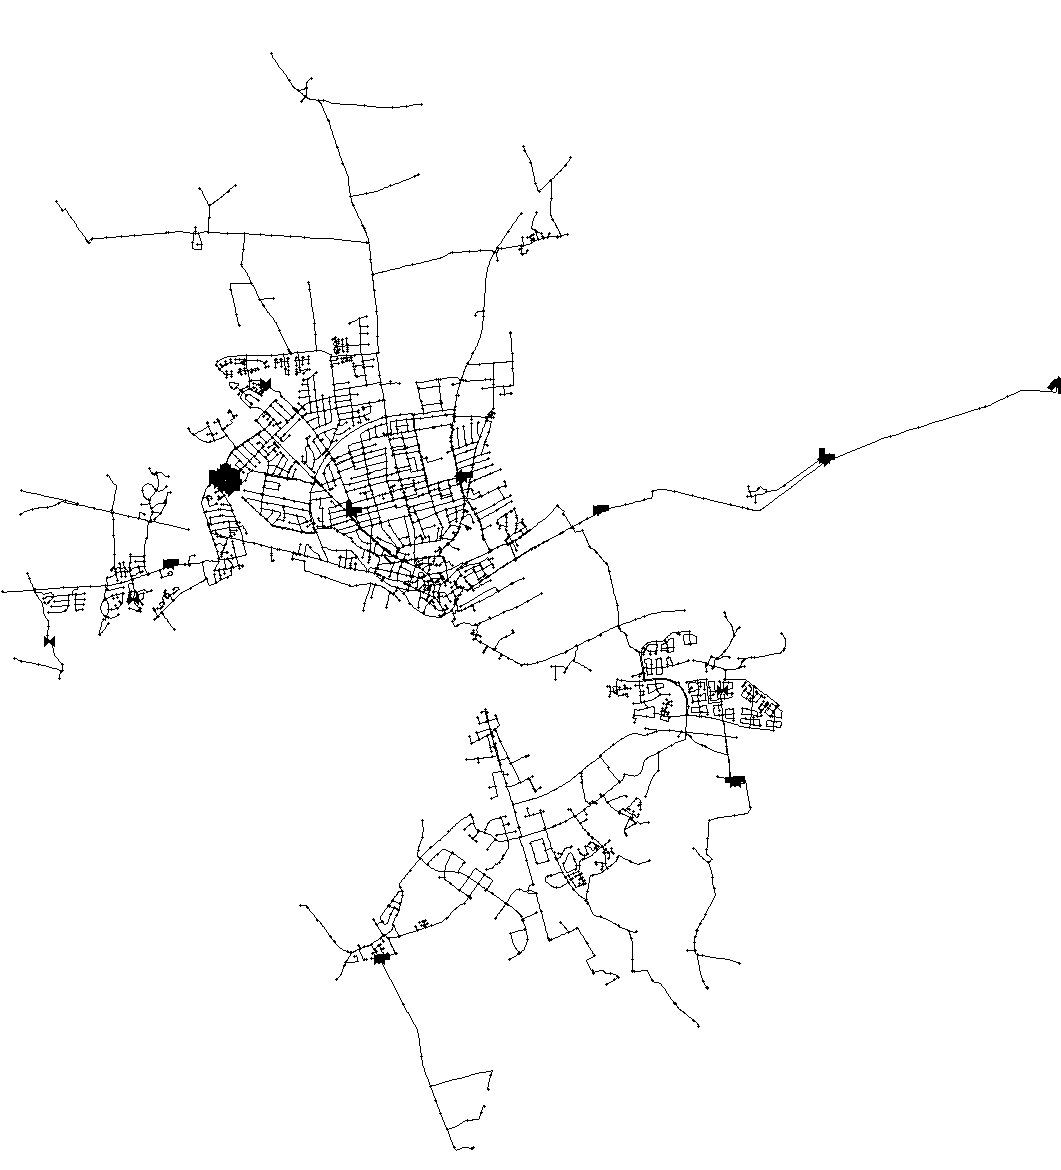
\includegraphics[width=1\textwidth]{report/pictures/verdo_pic}
 \usetikzlibrary{arrows}
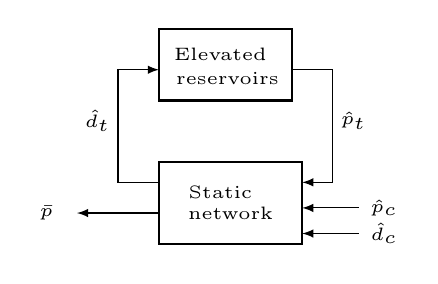
\begin{tikzpicture}[scale=1.3,transform shape]

\node at (-1.2,-2.5) {\tiny Static};
\node at (-1.1,-2.7) {\tiny network};
\node at (-1.2,-1.15) {\tiny Elevated};
\node at (-1.13,-1.38) {\tiny reservoirs};
\node at (0.1,-1.8) {\tiny $\hat{p}_t$};
\node at (-2.4,-1.8) {\tiny $\hat{d}_t$};
\node at (0.4,-2.65) {\tiny $\hat{p}_c$};
\node at (0.4,-2.9) {\tiny $\hat{d}_c$};
\node at (-2.9,-2.7) {\tiny $\bar{p}$};

\draw [thick] (-1.8,-0.9) rectangle (-0.5,-1.6);
\draw [thick] (-1.8,-2.2) rectangle (-0.4,-3);
\draw [-latex](-0.5,-1.3) -- (-0.1,-1.3) -- (-0.1,-2.4) -- (-0.4,-2.4);
\draw [-latex](0.15,-2.65) -- (-0.4,-2.65);
\draw [-latex](0.15,-2.9) -- (-0.4,-2.9);
\draw [-latex](-1.8,-2.4) -- (-2.2,-2.4) -- (-2.2,-1.3) -- (-1.8,-1.3);
\draw [-latex](-1.8,-2.7) -- (-2.6,-2.7);
\end{tikzpicture} 
\caption{Block diagram of the system with WTs.}
\label{fig:WT_system_blockdiagram}
\end{figure}

where the 'Elevated reservoirs' block has dynamics. The reservoirs act as integrators on the demand flow into or out of the tank. 

\newpage

\section{EPANET modelling}
\label{EPANET_modelling}

EPANET is an open source software, created by the United States Environmental Protection Agency (EPA) for simulating hydraulic networks \cite{agency2016epanet}. EPANET allows to track the flow of water in each pipe, the pressure at each node and the height of water in each tank. Furthermore, it uses a node-based model approach which means that the components in the network are either treated as nodes or links. Valves, pumps, reservoirs and tanks are considered as nodes due to their fixed geographical location and geodesic level. Pipes are considered as the links between the nodes in the network. Therefore, nodes are termination points for one or more pipes. The end-user consumption flow demand is considered as an attribute of certain nodes. Such nodes are called demand nodes and they have a certain water withdrawal. Attributes of nodes in the network are the geographical and geodesic coordinates, the flow demand, the total, and the available head. \cite{agency2016epanet}  

In EPANET, there is a function to carry out simulations within an extended period. Time patterns can be created that make demands at the nodes vary in a periodic way over the course of the time period. Nodal demands, reservoirs and pump schedules can all have time patterns associated with them, thus making the hydraulic simulation of the network more realistic. In order to create a schedule plan for changing reservoir levels or schedules for the pumping strategy, it is sufficient to have simulation data only at certain time steps. Therefore it is sufficient to solve the network using a set of hourly time steps (snapshots) over a period of 24 hours, and use the static, steady-state solutions for pump scheduling \cite{agency2016epanet}. The main function of EPANET is this, and therefore is used within this project for extended period analysis. During the analysis, pressure and flow values, along with the demand pattern can be simulated for periodic time steps. 

Since all nodes and links in the network have their unique IDs, during the project, the name of certain components will always have a reference to the original IDs in EPANET, for the better and clearer trackability. 









